\mySection{7.1 Introduction}
%-------------- start slide -------------------------------%{{{ 7.4.
\begin{frame}
% {\S\: 7.1 Introduction}
	\centering
		\begin{minipage}{0.4\textwidth}
\centering
		\includegraphics[scale=0.25]{Gauss.png}
		(1777-1855)
\end{minipage}
		\qquad
		\begin{minipage}{0.4\textwidth}
\centering
		\includegraphics[scale=0.25]{Laplace.png}
		(1749-1827)
\end{minipage}
\end{frame}
%-------------- end slide -------------------------------%}}}
%-------------- start slide -------------------------------%{{{ 7.5.
\begin{frame}
	\centering
	\begin{minipage}{0.28\textwidth}
		\centering
	\includegraphics[scale=0.23]{Normal_Distribution_PDF-neg.png}
\end{minipage}
% \hspace{3em}
\hfill
\begin{minipage}{0.63\textwidth}
	\centering
	\includegraphics[scale=0.13]{Normal_List_Properties-neg.png}
\end{minipage}
\vfill
\footnotesize
\url{https://en.wikipedia.org/wiki/Normal_distribution}
\end{frame}
%-------------- end slide -------------------------------%}}}
%-------------- start slide -------------------------------%{{{ 7.6.
\begin{frame}{Test for normal parameters (one sample test)}
\begin{enumerate}
	\item[Let] $Y_1,\cdots,Y_n$ be a random sample from $N(\mu,\sigma^2)$.
		\vfill
	\item[Prob. 1] Find a test statistic $\Lambda$ in order to test\hfill $H_0 : \mu = \mu_0$ v.s. $H_1 : \mu \ne \mu_0$. \\[2em]
	\item[]When $\sigma^2$ is known: \hspace{4em}
		$\displaystyle	\Lambda =  \frac{\overline{Y}-\mu_0}{\sigma/\sqrt{n}}\sim N(0,1)$\\[1em]
\item[] When $\sigma^2$ is unknown: \hspace{3em} $\displaystyle \Lambda = \alert{?}$
	\pause \hspace{3em}
	$\displaystyle	\Lambda \stackrel{\alert{?}}{=}  \frac{\overline{Y}-\mu_0}{s/\sqrt{n}}\quad \sim\quad \alert{?}$
	\vfill
	\item[Prob. 2] Find a test statistic $\Lambda$ in order to test\hfill $H_0 : \sigma^2 = \sigma_0^2$ v.s. $H_1 : \sigma^2 \ne \sigma^2_0$. \\[2em]
\end{enumerate}
\end{frame}
%-------------- end slide -------------------------------%}}}
%-------------- start slide -------------------------------%{{{ 7.7.
\begin{frame}
	\begin{enumerate}
	\item[Prob. 1] Find a test statistic for $H_0 : \mu = \mu_0$ v.s. $H_1 : \mu \ne \mu_0$, with $\sigma^2$ unknown\\[2em]
		\vfill
\item[Sol.] Composite-vs-composite test with:
\[\omega =\left\{(\mu,\sigma^2): \mu=\mu_0, \: \sigma^2>0\right\}\]
\[\Omega =\left\{(\mu,\sigma^2): \mu\in\R, \: \sigma^2>0\right\}\]\\[2em]
\item[] The MLE under the two spaces are:
	\begin{align}\tag{Under $\omega$}
		\omega_e=(\mu_e,\sigma_e^2): \qquad
		\mu_e =\mu_0	\quad\text{and}\quad \sigma_e^2 = \frac 1n \sum_{i=1}^n (y_i-\mu_0)^2
	\end{align}
	\begin{align}\tag{Under $\Omega$}
		\Omega_e=(\mu_e,\sigma_e^2): \qquad
		\mu_e =\bar{y}	\quad\text{and}\quad \sigma_e^2 = \frac 1n \sum_{i=1}^n (y_i-\bar{y})^2
	\end{align}
	\end{enumerate}
\end{frame}
%-------------- end slide -------------------------------%}}}
%-------------- start slide -------------------------------%{{{ 7.8.
\begin{frame}
	\begin{enumerate}
		\item[]
			\[
				L(\mu,\sigma^2) = (2\pi \sigma^2)^{-n} \exp \left( -\frac{1}{2} \sum_{i=1}^n \left(  \frac{y_i-\mu}{\sigma} \right)^2\right)
			\]
			\vfill
		\item[]	\[
				L(\omega_e) =  \cdots  = \left[  \frac{ne^{-1}}{2\pi\sum_{i=1}^n (y_i-\mu_0)^2}\right]^{n/2}
			\]
			\bigskip
			\[
				L(\Omega_e) =  \cdots  = \left[  \frac{ne^{-1}}{2\pi\sum_{i=1}^n (y_i-\bar{y})^2}\right]^{n/2}
			\]
		\end{enumerate}
\end{frame}
%-------------- end slide -------------------------------%}}}
%-------------- start slide -------------------------------%{{{ 7.9.
\begin{frame}

\begin{enumerate}
		\item[] Hence,
		\begin{align*}
			\lambda = \frac{L(\omega_e)}{L(\Omega_e)} & = \left[  \frac{\sum_{i=1}^n (y_i-\bar{y})^2}{\sum_{i=1}^n (y_i-\mu_0)^2}\right]^{n/2} = \cdots  = \left[ 1+ \frac{n(\bar{y}-\mu_0)^2}{\sum_{i=1}^n (y_i-\bar{y})^2}\right]^{-n/2} \\[2em]
                                                & = \left[ 1+ \frac{1}{n-1}\left(\frac{\bar{y}-\mu_0}{\sqrt{ \frac{1}{n-1}\sum_{i=1}^n (y_i-\bar{y})^2}\:\bigg/\:\sqrt{n}}\right)^2\right]^{-n/2}                                    \\[2em]
                                                & = \left[ 1+ \frac{1}{n-1}\left(\textcolor{magenta}{\frac{\bar{y}-\mu_0}{s\:/\:\sqrt{n} }}\right)^2\right]^{-n/2}                                                                    \\[2em]
                                                & = \left[ 1+ \frac{\textcolor{magenta}{t}^2}{n-1}\right]^{-n/2},\quad t= \frac{\bar{y}-\mu_0}{s\:/\:\sqrt{n}}
		\end{align*}
	\end{enumerate}
\end{frame}
%-------------- end slide -------------------------------%}}}
%-------------- start slide -------------------------------%{{{ Plot labmda(t) function
\begin{frame}[fragile]
\begin{center}
 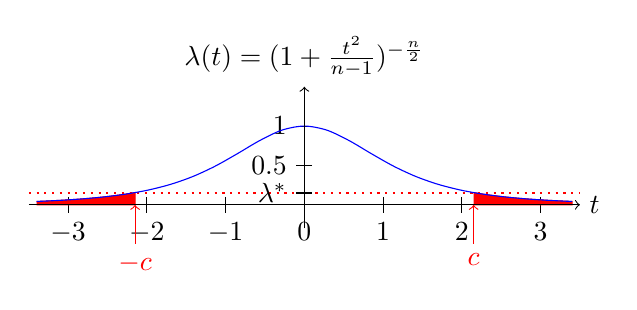
\begin{tikzpicture}
	 \def\n{4}
		\foreach \x in {-3,...,3}{
				\draw (\x,0.1)--++(0,-0.2) node [below] {$\x$};
		}
		\foreach \y in {0.5,1}{
				\draw (0.1,\y)--++(-0.2,0) node [left] {$\y$};
		}
		\def\level{0.15}
		\def\crt{2.15}
		\draw[red, dotted,thick] (-3.5, \level) -- (3.5, \level);
		\draw (-0.1,\level) node [left] {$\lambda^*$} -- (0.1,\level);
	 \filldraw[scale=1, domain= \crt: 3.4, smooth, variable=\t, red] plot ({\t}, {(1+\t*\t/(\n-1))^(-\n/2)}) -- (3.4,0) -- (\crt,0);
	 \filldraw[scale=1, domain=-3.4:-\crt, smooth, variable=\t, red] plot ({\t}, {(1+\t*\t/(\n-1))^(-\n/2)})-- (-\crt,0) -- (-3.4,0);
	 \draw [red, <-] (\crt,0) -- (\crt, -0.5) node [below] {$c$};
	 \draw [red, <-] (-\crt,0) -- (-\crt, -0.5) node [below] {$-c$};
	 \draw[scale=1, domain=-3.4:3.4, smooth, variable=\t, blue] plot ({\t}, {(1+\t*\t/(\n-1))^(-\n/2)});
   \draw[->] (-3.5, 0) -- (3.5, 0) node[right] {$t$};
	 \draw[->] (0, -0.3) -- (0, 1.5) node[above] {$\lambda(t)=(1+\frac{t^2}{n-1})^{-\frac{n}{2}}$};
 \end{tikzpicture}
 \bigskip

 \begin{align*}
	 \lambda\in (0,\lambda^*]	\qquad \Leftrightarrow \qquad |t| \ge c.
 \end{align*}
\end{center}
\end{frame}
%-------------- end slide -------------------------------%}}}
%-------------- start slide -------------------------------%{{{ 7.10.
\begin{frame}

	\begin{enumerate}
		\item[]Finally, the test statistic is \\[2em]
			\[
				\boxed{T =  \frac{\overline{Y}-\mu_0}{S/\sqrt{n}} }
			\]
			\\[2em]
			\[
				\text{with }\quad
				\overline{Y}= \frac 1n \sum_{i=1}^n Y_i
				\quad\text{and}\quad
				S^2 =  \frac{1}{n-1} \sum_{i=1}^n \left(Y_i-\overline{Y} \right)^2.
			\]
		\item[] The critical region takes the form: $|t|\ge c$.
		\vfill
		\item[] {\bf Question:~} Find the exact distribution of $T$.
	\end{enumerate}
\end{frame}
%-------------- end slide -------------------------------%}}}
%-------------- start slide -------------------------------%{{{ 7.11. Prob. 2
\begin{frame}
	\begin{enumerate}
	\item[Prob. 2] Find a test statistic for $H_0 : \sigma^2 = \sigma^2_0$ v.s. $H_1 : \sigma^2 \ne \sigma^2_0$, with $\mu$ unknown\\[2em]
		\vfill
	\item[Sol.] Composite-vs-composite test with:\\[1em]
\[\omega =\left\{(\mu,\sigma^2): \mu\in\R, \: \sigma^2=\sigma_0^2\right\}\]
\[\Omega =\left\{(\mu,\sigma^2): \mu\in\R, \: \sigma^2>0\right\}\]\\[2em]
\item[] The MLE under the two spaces are:\\[1em]
	\begin{align}\tag{Under $\omega$}
		\omega_e=(\mu_e,\sigma_e^2): \qquad
		\mu_e =\bar{y}	\quad\text{and}\quad \sigma_e^2 =\sigma_0^2\phantom{aaaaaaaaaa}
	\end{align}
	\begin{align}\tag{Under $\Omega$}
		\Omega_e=(\mu_e,\sigma_e^2): \qquad
		\mu_e =\bar{y}	\quad\text{and}\quad \sigma_e^2 = \frac 1n \sum_{i=1}^n (y_i-\bar{y})^2
	\end{align}
	\end{enumerate}
\end{frame}
%-------------- end slide -------------------------------%}}}
%-------------- start slide -------------------------------%{{{ 7.12.
\begin{frame}
	\begin{enumerate}
		\item[]
			\[
				L(\mu,\sigma^2) = (2\pi \sigma^2)^{-n} \exp \left( -\frac{1}{2} \sum_{i=1}^n \left(  \frac{y_i-\mu}{\sigma} \right)^2\right)
			\]
			\vfill
		\item[]	\[
				L(\omega_e) =  (2\pi \sigma^2)^{-n} \exp \left( -\frac{1}{2} \sum_{i=1}^n \left(  \frac{y_i-\bar{y}}{\sigma_0} \right)^2\right)
			\]
			\\[1em]
			\[
				L(\Omega_e) =  \cdots  = \left[  \frac{ne^{-1}}{2\pi\sum_{i=1}^n (y_i-\bar{y})^2}\right]^{n/2}
			\]
		\end{enumerate}
\end{frame}
%-------------- end slide -------------------------------%}}}
%-------------- start slide -------------------------------%{{{ 7.13.
\begin{frame}
\begin{enumerate}
		\item[] Hence,
		\begin{align*}
			\lambda & = \frac{L(\omega_e)}{L(\Omega_e)} = \left[  \frac{\sum_{i=1}^n (y_i-\bar{y})^2}{n\sigma_0^2}\right]^{n/2} \exp\left(- \frac{1}{2}\sum_{i=1}^n \left( \frac{y_i-\bar{y}}{\sigma_0} \right)^2 +\frac n2\right)                 \\[2em]
							& = \left[  \frac{\alert{\frac{1}{n-1}\sum_{i=1}^n (y_i-\bar{y})^2}}{ \frac{n}{n-1}\sigma_0^2}\right]^{n/2} \exp\left(- \frac{n-1}{2\sigma_0^2} \alert{\frac{1}{n-1}\sum_{i=1}^n \left( y_i-\bar{y}\right)^2} +\frac n2\right) \\[2em]
							& = \left[  \frac{ \alert{s^2}}{ \frac{n}{n-1}\sigma_0^2}\right]^{n/2} \exp\left(- \frac{n-1}{2\sigma_0^2} \alert{s^2} +\frac n2\right)
		\end{align*}
		\item[] \[\Downarrow\]
		\begin{align*}
			\lambda(s^2) = \left[  \frac{ s^2}{ \frac{n}{n-1}\sigma_0^2}\right]^{n/2} \exp\left(- \frac{n-1}{2\sigma_0^2} s^2 +\frac n2\right)
			\quad\Longleftrightarrow\quad v(s^2) = (s^2)^{\frac{n}{2}} e^{ -\lambda s^2 }
		\end{align*}
\end{enumerate}
\end{frame}
%-------------- end slide -------------------------------%}}}
%-------------- start slide -------------------------------%{{{ 1 v(s) function plot
\begin{frame}[fragile]
\begin{center}
	By setting $n=6$ and  $\lambda=0.8$,  we see ...\\[1em]

	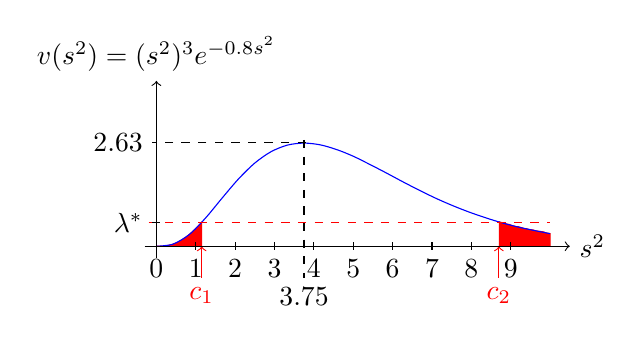
\begin{tikzpicture}[scale=0.5]
  % \filldraw[scale=1, domain=3.7:3.8, smooth, variable=\x, green] plot ({\x}, {\x*\x*\x*exp(-0.8*\x)}) -- (3.8,2.6248) -- (3.7,2.6248);
	\def\left{1.15}
  \filldraw[scale=1, domain=0:\left, smooth, variable=\x, red] plot ({\x}, {\x*\x*\x*exp(-0.8*\x)}) -- (\left,0) -- (0,0);
	\def\right{8.7}
  \filldraw[scale=1, domain=\right:10, smooth, variable=\x, red] plot ({\x}, {\x*\x*\x*exp(-0.8*\x)}) -- (10,0) -- (\right,0);
  \draw[scale=1, domain=0:10, smooth, variable=\x, blue] plot ({\x}, {\x*\x*\x*exp(-0.8*\x)});
	\foreach \x in {0,...,9}{
			\draw (\x,0.1)--++(0,-0.2) node [below] {$\x$};
	}
	\draw[dashed] (3.75,2.7) -- (3.75,-0.8) node [below] {$3.75$};
	\draw[dashed] (3.8,2.6255) -- (-0.1,2.6255) node [left] {$2.63$};
	\def\level{0.6}
	\draw[dashed,red] (-0.2,\level) -- (10,\level);
	\draw[red,<-] (\left,0) -- (\left, -0.8) node [below] {$c_1$};
	\draw[red,<-] (\right,0) -- (\right, -0.8) node [below] {$c_2$};
	\draw (-0.1,\level) node [left] {$\lambda^*$} -- (0.1,\level);
  \draw[->] (-0.3, 0) -- (10.5, 0) node[right] {$s^2$};
  \draw[->] (0, -0.3) -- (0, 4.2) node[above] {$v(s^2)=(s^2)^3e^{-0.8s^2}$};
	\end{tikzpicture}

	\vfill

	This suggests that the critical region should be of the form in terms of $s^2$:
	\begin{align*}
		(0,c_1) \cup (c_2,\infty)
	\end{align*}
	For convenience, we put $\alpha/2$ mass on each tails of $S^2$:\\[1em]
	Find $c_1$ and $c_2$ such that
	\begin{align*}
		\int_0^{c_1} f_{S^2}(z)dz = \int_{c_2}^\infty f_{S^2}(z)dz = \frac{\alpha}{2}.
	\end{align*}
\end{center}
\end{frame}
%-------------- end slide -------------------------------%}}}
%-------------- start slide -------------------------------%{{{ 7.14.
\begin{frame}
	\begin{enumerate}
		\item[]Finally, the test statistic is \\[2em]
			\[
				\boxed{S^2 = \frac{1}{n-1}\sum_{i=1}^n \left( Y_i-\overline{Y}\right)^2}
				\quad \text{with }\quad
				\overline{Y}= \frac 1n \sum_{i=1}^n Y_i
			\]
		\vfill
		\item[] {\bf Question:~} Find the exact distribution of $S^2$.
	\end{enumerate}
\end{frame}
%-------------- end slide -------------------------------%}}}
